\documentclass[12pt]{article}
\usepackage[utf8]{inputenc}
\usepackage{float}
\usepackage{amsmath}


\usepackage[hmargin=3cm,vmargin=6.0cm]{geometry}
%\topmargin=0cm
\topmargin=-2cm
\addtolength{\textheight}{6.5cm}
\addtolength{\textwidth}{2.0cm}
%\setlength{\leftmargin}{-5cm}
\setlength{\oddsidemargin}{0.0cm}
\setlength{\evensidemargin}{0.0cm}

%misc libraries goes here
\usepackage{tikz}
\usetikzlibrary{automata,positioning}

\begin{document}

\section*{Student Information } 
%Write your full name and id number between the colon and newline
%Put one empty space character after colon and before newline
Full Name : Koray Can YURTSEVEN \\
Id Number : 2099547 \\

% Write your answers below the section tags
\section*{Answer 1}

\subsection*{a.}

\begin{table}[H]
\centering
\caption{Rules after removing e transition}
\begin{tabular}{lll}
                 &       & Rule of G \\
S-\textgreater{} & aSXaX & R1        \\
S-\textgreater{} & aSaX  & R2        \\
S-\textgreater{} & aSXa  & R3        \\
S-\textgreater{} & aSa   & R4        \\
S-\textgreater{} & bSXbX & R5        \\
S-\textgreater{} & bSbX  & R6        \\
S-\textgreater{} & bSXb  & R7        \\
S-\textgreater{} & bSb   & R8        \\
S-\textgreater{} & c     & R9        \\
X-\textgreater{} & aX    & R10       \\
X-\textgreater{} & a     & R11       \\
X-\textgreater{} & bX    & R12       \\
X-\textgreater{} & b     & R13      
\end{tabular}
\end{table}

Note that, I have removed $e$ transitions for simplicity.\\

\begin{table}[H]
\centering
\caption{Transitions}
\begin{tabular}{lll}
Transition Left Side & Transition Right Side & Transition Name \\
(p,a,e)              & (p,a)                 & T0              \\
(p,e,XaXSa)          & (p,S)                 & T1              \\
(p,e,XaSa)           & (p,S)                 & T2              \\
(p,e,aXSa)           & (p,S)                 & T3              \\
(p,e,aSa)            & (p,S)                 & T4              \\
(p,e,XbXSb)          & (p,S)                 & T5              \\
(p,e,XbSb)           & (p,S)                 & T6              \\
(p,e,bXSb)           & (p,S)                 & T7              \\
(p,e,bSb)            & (p,S)                 & T8              \\
(p,e,c)              & (p,S)                 & T9              \\
(p,e,Xa)             & (p,X)                 & T10             \\
(p,e,a)              & (p,X)                 & T11             \\
(p,e,Xb)             & (p,X)                 & T12             \\
(p,e,b)              & (p,X)                 & T13             \\
(p,e,S)              & (q,e)                 & T14            
\end{tabular}
\end{table}

\subsection*{b.}

\begin{table}[H]
\centering
\caption{Solution for w = abbcbabbaa}
\begin{tabular}{llllll}
Step & State & Unread     & Stack & Transition Used & Rule of G \\
0    & p     & abbcbabbaa & e     & -               & -         \\
1    & p     & bbcbabbaa  & a     & T0              & -         \\
2    & p     & bcbabbaa   & ba    & T0              & -         \\
3    & p     & cbabbaa    & bba   & T0              & -         \\
4    & p     & babbaa     & cbba  & T0              & -         \\
5    & p     & babbaa     & Sbba  & T9              & R9        \\
6    & p     & abbaa      & bSbba & T0              & -         \\
7    & p     & abbaa      & Sba   & T8              & R8        \\
8    & p     & bbaa       & aSba  & T0              & -         \\
9    & p     & baa        & baSba & T0              & -         \\
10   & p     & baa        & XaSba & T13             & R13       \\
11   & p     & baa        & XSba  & T10             & R10       \\
12   & p     & aa         & bXSba & T0              & -         \\
13   & p     & aa         & Sa    & T7              & R7        \\
14   & p     & a          & aSa   & T0              & -         \\
15   & p     & a          & XSa   & T11             & R11       \\
16   & p     & e          & aXSa  & T0              & -         \\
17   & p     & e          & S     & T3              & R3        \\
18   & q     & e          & e     & T14             & -        
\end{tabular}
\end{table}

\section*{Answer 2}

\subsection*{a.}

\begin{table}[H]
\centering
\caption{Solution of TM for q2.a}
\begin{tabular}{|l|l|l|}
\hline
\begin{tabular}[c]{@{}l@{}}Current state \\ and \\ symbol read\end{tabular} & \begin{tabular}[c]{@{}l@{}}Next state \\ and \\ symbol changed\end{tabular} & Description                                                                                                                                                                                                  \\ \hline
qi,U                                                                        & qo,-\textgreater{}                                                          & Initial, move right to read first character                                                                                                                                                                  \\ \hline
q0,1                                                                        & q1,-\textgreater{}                                                          & If we read 1, change state and move head to right                                                                                                                                                            \\ \hline
q1,1                                                                        & q0,-\textgreater{}                                                          & \begin{tabular}[c]{@{}l@{}}Oscilate between q0 and q1 till we face blank \\ character\end{tabular}                                                                                                           \\ \hline
q1,U                                                                        & qh,1                                                                        & \begin{tabular}[c]{@{}l@{}}When we encounter with blank character,\\ if we are in state q1, that means the length of\\ the string is odd. Place the current position to 1,\\ and finish reading\end{tabular} \\ \hline
q0,U                                                                        & q2,\textless{}-                                                             & String length is even, Change state and go left                                                                                                                                                              \\ \hline
q2,1                                                                        & q2,\textless{}-                                                             & Go left till find blank at the beginning                                                                                                                                                                     \\ \hline
q2,U                                                                        & q3,-\textgreater{}                                                          & We've reached the beginning. Go one right                                                                                                                                                                    \\ \hline
q3,1                                                                        & q3,0                                                                        & Change 1 to 0, stay at the current position                                                                                                                                                                  \\ \hline
q3,0                                                                        & q4,-\textgreater{}                                                          & \begin{tabular}[c]{@{}l@{}}If we see 0 in q3, change state q4 and find the\\ end of the input\end{tabular}                                                                                                   \\ \hline
q4,1                                                                        & q4,-\textgreater{}                                                          & See above                                                                                                                                                                                                    \\ \hline
q4,U                                                                        & q5,\textless{}-                                                             & \begin{tabular}[c]{@{}l@{}}When we reached the right end of the input,\\ go one left and make your state q5\end{tabular}                                                                                     \\ \hline
q5,1                                                                        & q5,U                                                                        & \begin{tabular}[c]{@{}l@{}}If we are in q5, make the current char. blank.\\ In this way we are deleting half of 1's at each\\ iteration\end{tabular}                                                         \\ \hline
q5,U                                                                        & q6,\textless{}-                                                             & Go left till find 0                                                                                                                                                                                          \\ \hline
q6,1                                                                        & q6,\textless{}-                                                             & Go left till find 0                                                                                                                                                                                          \\ \hline
q6,0                                                                        & q7,-\textgreater{}                                                          & \begin{tabular}[c]{@{}l@{}}We have found the first 0 from right. Go one\\ right and loop\end{tabular}                                                                                                        \\ \hline
q7,1                                                                        & q7,0                                                                        & Make the current char 0                                                                                                                                                                                      \\ \hline
q7,0                                                                        & q3,0                                                                        & Loop                                                                                                                                                                                                         \\ \hline
q7,U                                                                        & q8,\textless{}-                                                             & \begin{tabular}[c]{@{}l@{}}When we finished the loop, we are in q7,U\\ transition. Make our state q8 to go at the beginning\\ of the input to change 0's to 1's.\end{tabular}                                \\ \hline
q8,0                                                                        & q8,\textless{}-                                                             & Find the beginning of the string                                                                                                                                                                             \\ \hline
q8,U                                                                        & q9,-\textgreater{}                                                          & Make state q9 and go right to change 0's to 1's                                                                                                                                                              \\ \hline
q9,0                                                                        & q9,1                                                                        &                                                                                                                                                                                                              \\ \hline
q9,1                                                                        & q9,-\textgreater{}                                                          &                                                                                                                                                                                                              \\ \hline
q9,U                                                                        & qh,U                                                                         & \begin{tabular}[c]{@{}l@{}}We have converted all 0's to 1's. We have restored\\ the string in problem definition's format. We\\ are done\end{tabular}                                                        \\ \hline
\end{tabular}
\end{table}

\section*{Answer 3}

Given transition rule $\delta(q,x) = (p,y,d)$ where $q$ is the current state, $x$ is the content of the current cell, $p$ is the new state, $y$ is the replacing symbol and $d$ is the direction, when we move only to the right, $d$ becomes irrelevant. Also, it is unnecessary to overwrite something because we always move to the right. Even if we write over something, that becomes useless. Therefore we can ignore $y$ and $d$. Hence, we will have $\delta(q,x) = (p)$, i.e. transition for Finite Automata.

\section*{Answer 4}

\subsection*{a.}
A queue machine can be defined as a five tuple:\\
$M = (K,\Sigma, \delta, s, H)$ where,
\\
$K$ is a finite set of states,\\
$\Sigma$ is the finite set of the input alphabet, plus blank character and the starting symbol\\
$s$ is the initial state, and it is an element of $K$,\\
$H \in K$ is the halting state,\\
$\delta$ is a transition function from all of the states except the halting states with reading an input to all of the states with reading an element, plus (up, element),(down, element), (right, element), (left, element), where:\\
$left$ is front\\
$right$ is rear\\
$up$ is enqueue\\
and the $down$ is dequeue\\

\subsection*{b.}

\subsection*{c.}

\subsection*{d.}
They are equivalent because:\\
$i)$ Accessing front element in queue TM, go left until reaching the start symbol and after reaching the start symbol, go one element right.\\
$ii)$ Accesing rear element in queue TM, go right until reaching the blank symbol and after reaching the blank symbol, go one element left.\\
$iii)$ For enqueuing an element in queue TM, go right until reaching the blank symbol, replace the blank symbol with the element.\\
$iv)$ For dequeueing an element in queue TM, we can move the start point to one right position or we can shift all the element to the left by one position.\\
Note that the actions above are in the standard TM.\\
$v$ For going left and right in the standard TM, just use dequeue and enqueue in queue TM.\\

\subsection*{e.}

\section*{Answer 5}

\subsection*{a.}

\begin{center}
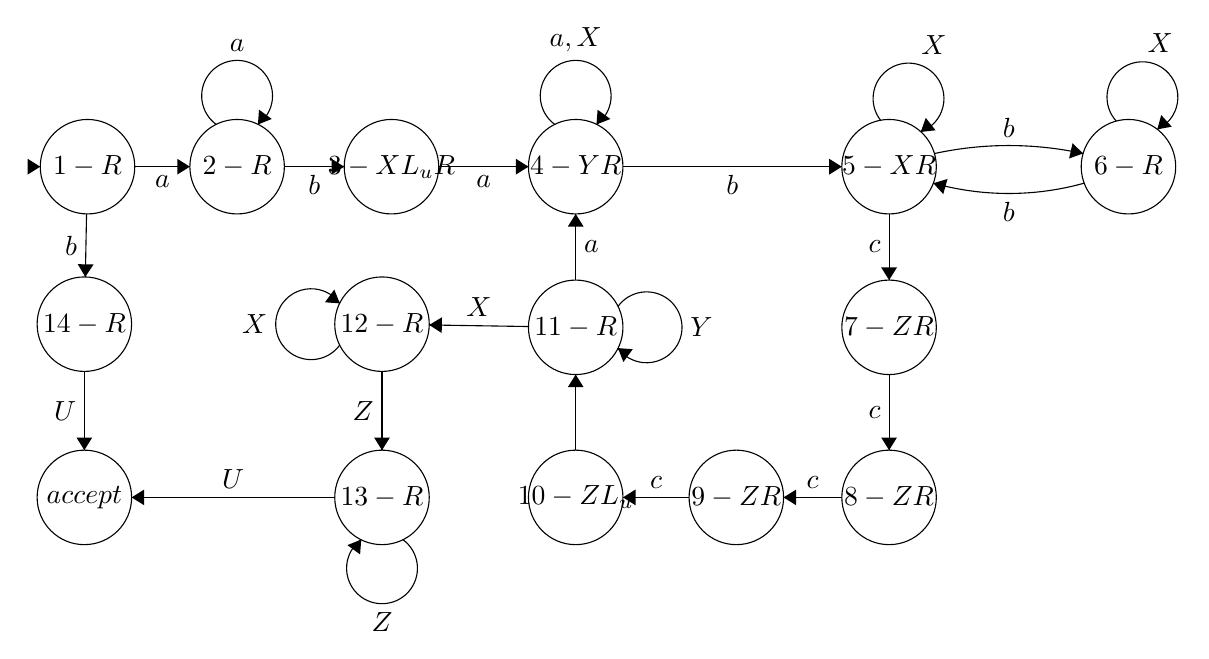
\begin{tikzpicture}[scale=0.2]
\tikzstyle{every node}+=[inner sep=0pt]
\draw [black] (5.2,-20.8) circle (3);
\draw (5.2,-20.8) node {$1-R$};
\draw [black] (14.7,-20.8) circle (3);
\draw (14.7,-20.8) node {$2-R$};
\draw [black] (24.5,-20.8) circle (3);
\draw (24.5,-20.8) node {$3-XL_uR$};
\draw [black] (36.2,-20.8) circle (3);
\draw (36.2,-20.8) node {$4-YR$};
\draw [black] (56.1,-20.8) circle (3);
\draw (56.1,-20.8) node {$5-XR$};
\draw [black] (71.3,-20.8) circle (3);
\draw (71.3,-20.8) node {$6-R$};
\draw [black] (56.1,-31) circle (3);
\draw (56.1,-31) node {$7-ZR$};
\draw [black] (56.1,-41.8) circle (3);
\draw (56.1,-41.8) node {$8-ZR$};
\draw [black] (46.4,-41.8) circle (3);
\draw (46.4,-41.8) node {$9-ZR$};
\draw [black] (36.2,-41.8) circle (3);
\draw (36.2,-41.8) node {$10-ZL_u$};
\draw [black] (36.2,-31) circle (3);
\draw (36.2,-31) node {$11-R$};
\draw [black] (23.9,-30.8) circle (3);
\draw (23.9,-30.8) node {$12-R$};
\draw [black] (23.9,-41.8) circle (3);
\draw (23.9,-41.8) node {$13-R$};
\draw [black] (5,-30.8) circle (3);
\draw (5,-30.8) node {$14-R$};
\draw [black] (5,-41.8) circle (3);
\draw (5,-41.8) node {$accept$};
\draw [black] (13.377,-18.12) arc (234:-54:2.25);
\draw (14.7,-13.55) node [above] {$a$};
\fill [black] (16.02,-18.12) -- (16.9,-17.77) -- (16.09,-17.18);
\draw [black] (34.877,-18.12) arc (234:-54:2.25);
\draw (36.2,-13.55) node [above] {$a,X$};
\fill [black] (37.52,-18.12) -- (38.4,-17.77) -- (37.59,-17.18);
\draw [black] (55.564,-17.86) arc (218.06854:-69.93146:2.25);
\draw (58.94,-13.74) node [above] {$X$};
\fill [black] (58.11,-18.59) -- (59.05,-18.49) -- (58.43,-17.7);
\draw [black] (70.532,-17.912) arc (222.61812:-65.38188:2.25);
\draw (73.32,-13.58) node [above] {$X$};
\fill [black] (73.13,-18.43) -- (74.05,-18.26) -- (73.38,-17.52);
\draw [black] (58.979,-19.965) arc (102.30317:77.69683:22.156);
\fill [black] (68.42,-19.96) -- (67.75,-19.31) -- (67.53,-20.28);
\draw (63.7,-18.96) node [above] {$b$};
\draw [black] (68.492,-21.845) arc (-74.40427:-105.59573:17.823);
\fill [black] (58.91,-21.85) -- (59.54,-22.54) -- (59.81,-21.58);
\draw (63.7,-23) node [below] {$b$};
\draw [black] (39.2,-20.8) -- (53.1,-20.8);
\fill [black] (53.1,-20.8) -- (52.3,-20.3) -- (52.3,-21.3);
\draw (46.15,-21.3) node [below] {$b$};
\draw [black] (27.5,-20.8) -- (33.2,-20.8);
\fill [black] (33.2,-20.8) -- (32.4,-20.3) -- (32.4,-21.3);
\draw (30.35,-21.3) node [below] {$a$};
\draw [black] (17.7,-20.8) -- (21.5,-20.8);
\fill [black] (21.5,-20.8) -- (20.7,-20.3) -- (20.7,-21.3);
\draw (19.6,-21.3) node [below] {$b$};
\draw [black] (8.2,-20.8) -- (11.7,-20.8);
\fill [black] (11.7,-20.8) -- (10.9,-20.3) -- (10.9,-21.3);
\draw (9.95,-21.3) node [below] {$a$};
\draw [black] (1.7,-20.8) -- (2.2,-20.8);
\fill [black] (2.2,-20.8) -- (1.4,-20.3) -- (1.4,-21.3);
\draw [black] (56.1,-23.8) -- (56.1,-28);
\fill [black] (56.1,-28) -- (56.6,-27.2) -- (55.6,-27.2);
\draw (55.6,-25.9) node [left] {$c$};
\draw [black] (56.1,-34) -- (56.1,-38.8);
\fill [black] (56.1,-38.8) -- (56.6,-38) -- (55.6,-38);
\draw (55.6,-36.4) node [left] {$c$};
\draw [black] (53.1,-41.8) -- (49.4,-41.8);
\fill [black] (49.4,-41.8) -- (50.2,-42.3) -- (50.2,-41.3);
\draw (51.25,-41.3) node [above] {$c$};
\draw [black] (43.4,-41.8) -- (39.2,-41.8);
\fill [black] (39.2,-41.8) -- (40,-42.3) -- (40,-41.3);
\draw (41.3,-41.3) node [above] {$c$};
\draw [black] (38.88,-29.677) arc (144:-144:2.25);
\draw (43.45,-31) node [right] {$Y$};
\fill [black] (38.88,-32.32) -- (39.23,-33.2) -- (39.82,-32.39);
\draw [black] (36.2,-28) -- (36.2,-23.8);
\fill [black] (36.2,-23.8) -- (35.7,-24.6) -- (36.7,-24.6);
\draw (36.7,-25.9) node [right] {$a$};
\draw [black] (36.2,-38.8) -- (36.2,-34);
\fill [black] (36.2,-34) -- (35.7,-34.8) -- (36.7,-34.8);
\draw [black] (5.14,-23.8) -- (5.06,-27.8);
\fill [black] (5.06,-27.8) -- (5.58,-27.01) -- (4.58,-26.99);
\draw (4.57,-25.8) node [left] {$b$};
\draw [black] (5,-33.8) -- (5,-38.8);
\fill [black] (5,-38.8) -- (5.5,-38) -- (4.5,-38);
\draw (4.5,-36.3) node [left] {$U$};
\draw [black] (33.2,-30.95) -- (26.9,-30.85);
\fill [black] (26.9,-30.85) -- (27.69,-31.36) -- (27.71,-30.36);
\draw (30.06,-30.38) node [above] {$X$};
\draw [black] (21.22,-32.123) arc (-36:-324:2.25);
\draw (16.65,-30.8) node [left] {$X$};
\fill [black] (21.22,-29.48) -- (20.87,-28.6) -- (20.28,-29.41);
\draw [black] (23.9,-33.8) -- (23.9,-38.8);
\fill [black] (23.9,-38.8) -- (24.4,-38) -- (23.4,-38);
\draw (23.4,-36.3) node [left] {$Z$};
\draw [black] (25.223,-44.48) arc (54:-234:2.25);
\draw (23.9,-49.05) node [below] {$Z$};
\fill [black] (22.58,-44.48) -- (21.7,-44.83) -- (22.51,-45.42);
\draw [black] (20.9,-41.8) -- (8,-41.8);
\fill [black] (8,-41.8) -- (8.8,-42.3) -- (8.8,-41.3);
\draw (14.45,-41.3) node [above] {$U$};
\end{tikzpicture}
\end{center}

Let me explain the notations above. Since I couldn't draw Turing Machine, I draw Finite Automaton and give each circle a number. Normally, there shouldn't be a number and a circle, but these are for clarifying my solutions. It is easy to draw finite automaton.Also, I didn't include the transition that corresponds to the "no" state. All transitions that are not listed above yields to "no" states. If I draw those transitions, my graph will be very complicated.\\
First, I assume that the given Turing Machine tape will be like in the following: $SUabbcccUU...$ where $S$ denotes start, $U$ denotes blank character, and rest are the string. \\
When we start at circle number one, we immediately move head to the right and start read the character under the head.\\
There are 2 options. If we read a $b$, we move to the circle 14 and move Right. And if read a blank character in here, that means we have reached the end of the input. We can accept this state. This string consists of only $b$.\\
Second option is we saw $a$. Then move in second circle. Whenever we see an $a$, we move head to the right. When we see a $b$, we move to the 3rd circle.\\
We replace this $b$ with $X$ and we do transition $L_u$ to find beginning of the string. When we reached the beginning of the string, we move right, under the head, there will be an $a$.\\
When we read an $a$, we move to the 4th circle, and we are replacing the current character, aka the $a$ with Y. In the 4th circle, whenever I see an $a$ or an $X$, I move to the right. I'm not replacing read symbols with $Y$. I'm only looping over the R symbol, which moves head to the right. Whenever I see a $b$, I move to the 5th circle.\\
In the 5th circle, when we are in the first iteration, we have 2 choice. The remaining characters are consist of $b$'s and $c$'s. Also, since we marked the first $b$ with an $X$, if the given string is correct, we should have $(2^n - 1)$ $b$'s in the string now. i.e. If I have 8 $b$ in the string at first, before I visit 5th circle, I must have 7 $b$'s. In the 5th circle, I change my $b$ to $X$, then if I see a $b$, I move to the 6th circle. In 6th circle, I skip $X$'s and when I see a $b$, I mark it as an $X$ and move to the 5th state.\\
One thing to mention here is that, when I do this loop in 2nd time, the square loop consists of 4-5-6-7-8-9-10-11-4, I have some $X$'s and some $b$'s in my string. Therefore I need to do a transition between 5 and 6 to skip those $X$'s. Also, every time I run over this loop, I'm marking half of the $b$'s with $X$. Since I have marked first $b$ in the 3rd circle, I have guaranteed that $(2^n -1)$ $b$ will end in $n$ cycles.\\
In the 5th cycle, when I have finish $b$'s, I should have encounter with a $c$. So for every $a$, I should have change 3 $c$'s into $Z$'s and move right to read next $c$.\\
In the 10th circle, I have finished marking 3 $c$, so I should go to the beginning of the string.\\
In the 11th circle, I'm going right to find the first $a$. If I find an $a$, I mark that $a$ as a $Y$, and do the loop 4-5-6-7-8-9-10-11-4. In this loop, for every $a$, I delete half of the $b$'s, and 3 $c$.\\
Again in the 11th circle, if I didn't encounter with an $a$ after I skipped $Y$'s, if the given string is correct, I expect that the character under the head must be a $X$, aka former $b$.\\
So, in circles 12 and 13, if the given string is correct, my string should be consist of as: YYXXXXZZZZZZ. I go right to find an blank character. When I find a blank character, it means that the given string is in the language, and the Turing Machine accepts that string.\\
The not drawn transitions always lead us to the not accepting state. For example, in the middle of conversion of my $b$'s to $X$'s, if I see an $a$, given string is not acceptable. It should go to the "no" state and halts. Also, while reading 3 consecutive $c$'s, I'm not expecting any character other than $c$.\\
In the 11th circle, if I don't encounter with an $a$, my string must be consist of $Y$'s, $X$'s and $Z$'s only. If any $a,b,c$ character  stayed in those states, that means the string is not in the language. While reading in 12 and 13, if I encounter with any of those characters, the machine must halt and reject the given string.\\ 

\subsection*{b.}



\section*{Answer 6}

\subsection*{a.}

Since $L_1 , L_2 , L_3$ are regular or context free languages, they can be represented by a machine.\\

In the forth point, if there is a TM that decides the given language, then there is also a TM that decides complement of $L_4$. Because it is decidable it is a recursive language. Also its complement $L_4$ (complement of complement of $L_4$) is also a recursive language. Therefore we can find a machine that accepts this language.\\

In the fifth point, since it is generated by a grammar, it is a recursively enumerable language. We can find a machine that accepts this language.\\

$M_1 , M_2 , M_3 , M_4 , M_5$ exist.\\

\subsection*{b.}

Yes, since they are accepted by Turing Machines, we can find an algorithm for membership problems associated with them.\\

\subsection*{c.}

\subsection*{d.}
No, not always. Recursively enumerable languages (semi-decidable) are not closed under complement.\\
RE promises us an acceptor, not a decider. Therefore, if we flip the machine, we'll have a machine that says "no" for the word is not in the language but loop otherwise. That is not a RE.\\
Also, proof by contradiction:\\
1- If L and its complement are both semi-decidable, then both are decidable.\\
2- Hence, if RE is closed under complement, we'll have R=RE.\\
3- But, it must R $\subset$ RE (by halting problem, it is semi-decidable), so it is a contradiction.

%Do not submit solutions for Question 7, yet do solve it.


\end{document}

​
